\documentclass{beamer}

\usepackage{beamerposter}
\usepackage[arrowdel]{physics}
\usepackage{siunitx}
\usepackage{amsmath}
\usepackage{amssymb}
\usepackage{graphicx}
\usepackage{subcaption}
%% \usepackage[hidelinks]{hyperref}
\usepackage{cleveref}

\setlength{\paperwidth}{24in}
\setlength{\paperheight}{36in}
\setlength{\textwidth}{23in}

%% For the Hindmarsh-Rose model
\newcommand{\hrx}{x}
\newcommand{\hry}{y}
\newcommand{\hrz}{z}
\newcommand{\hra}{\alpha}
\newcommand{\hrb}{\beta}

%% For the chimera-like index
\newcommand{\chimera}{\chi}
\newcommand{\meta}{m}
\newcommand{\ordparam}{r}
\newcommand{\phase}{\phi}

\title[UVM Student Research Conference, 17 April 2019, Burlington, VT]{Chimera States \& Seizures in a Mouse Neuronal Model}
\author{Henry Mitchell\inst{1,2,5},
  Peter Dodds\inst{1,4,5},
  Matt Mahoney\inst{3,4},
  Chris Danforth\inst{1,4,5}
}

\institute{
  \inst{1} Department of Mathematics and Statistics
  \inst{2} Department of Physics
  \inst{3} Department of Neurology \\
  \inst{4} Department of Computer Science
  \inst{5} Computational Story Lab
}

\usetheme{SRC}

\begin{document}

\begin{frame}[t]

  \begin{multicols}{3}

    \section{Abstract}
    \textbf{Chimera states}--- the coexistence of synchrony and asynchrony in a nonlocally-coupled network of identical oscillators—are often sought as a model for epileptic \textbf{seizures}.
    This work investigates that connection, seeking chimera states in a network of modified Hindmarsh-Rose neurons connected in the graph of the mesoscale mouse connectome.
    The model was found to be of sufficient quality to produce superficially epileptiform activity.
    The limitations of the model were investigated, depending on the strength of connections between subcortices within a cortex and between cortices.
    A wide swath of parameter space revealed persistent chimera states.


    \section{Chimera states}
    The coexistence of synchrony and asynchrony in a network of identical nonlocally coupled oscillators is called a \textbf{chimera state} \cite{Kuramoto2002,Abrams2004}.
    \Cref{fig:abrams} shows an example with a pair of populations, one synchronous and the other asynchronous.
    \begin{figure}
      \begin{subfigure}{0.66\columnwidth}
        \centering
        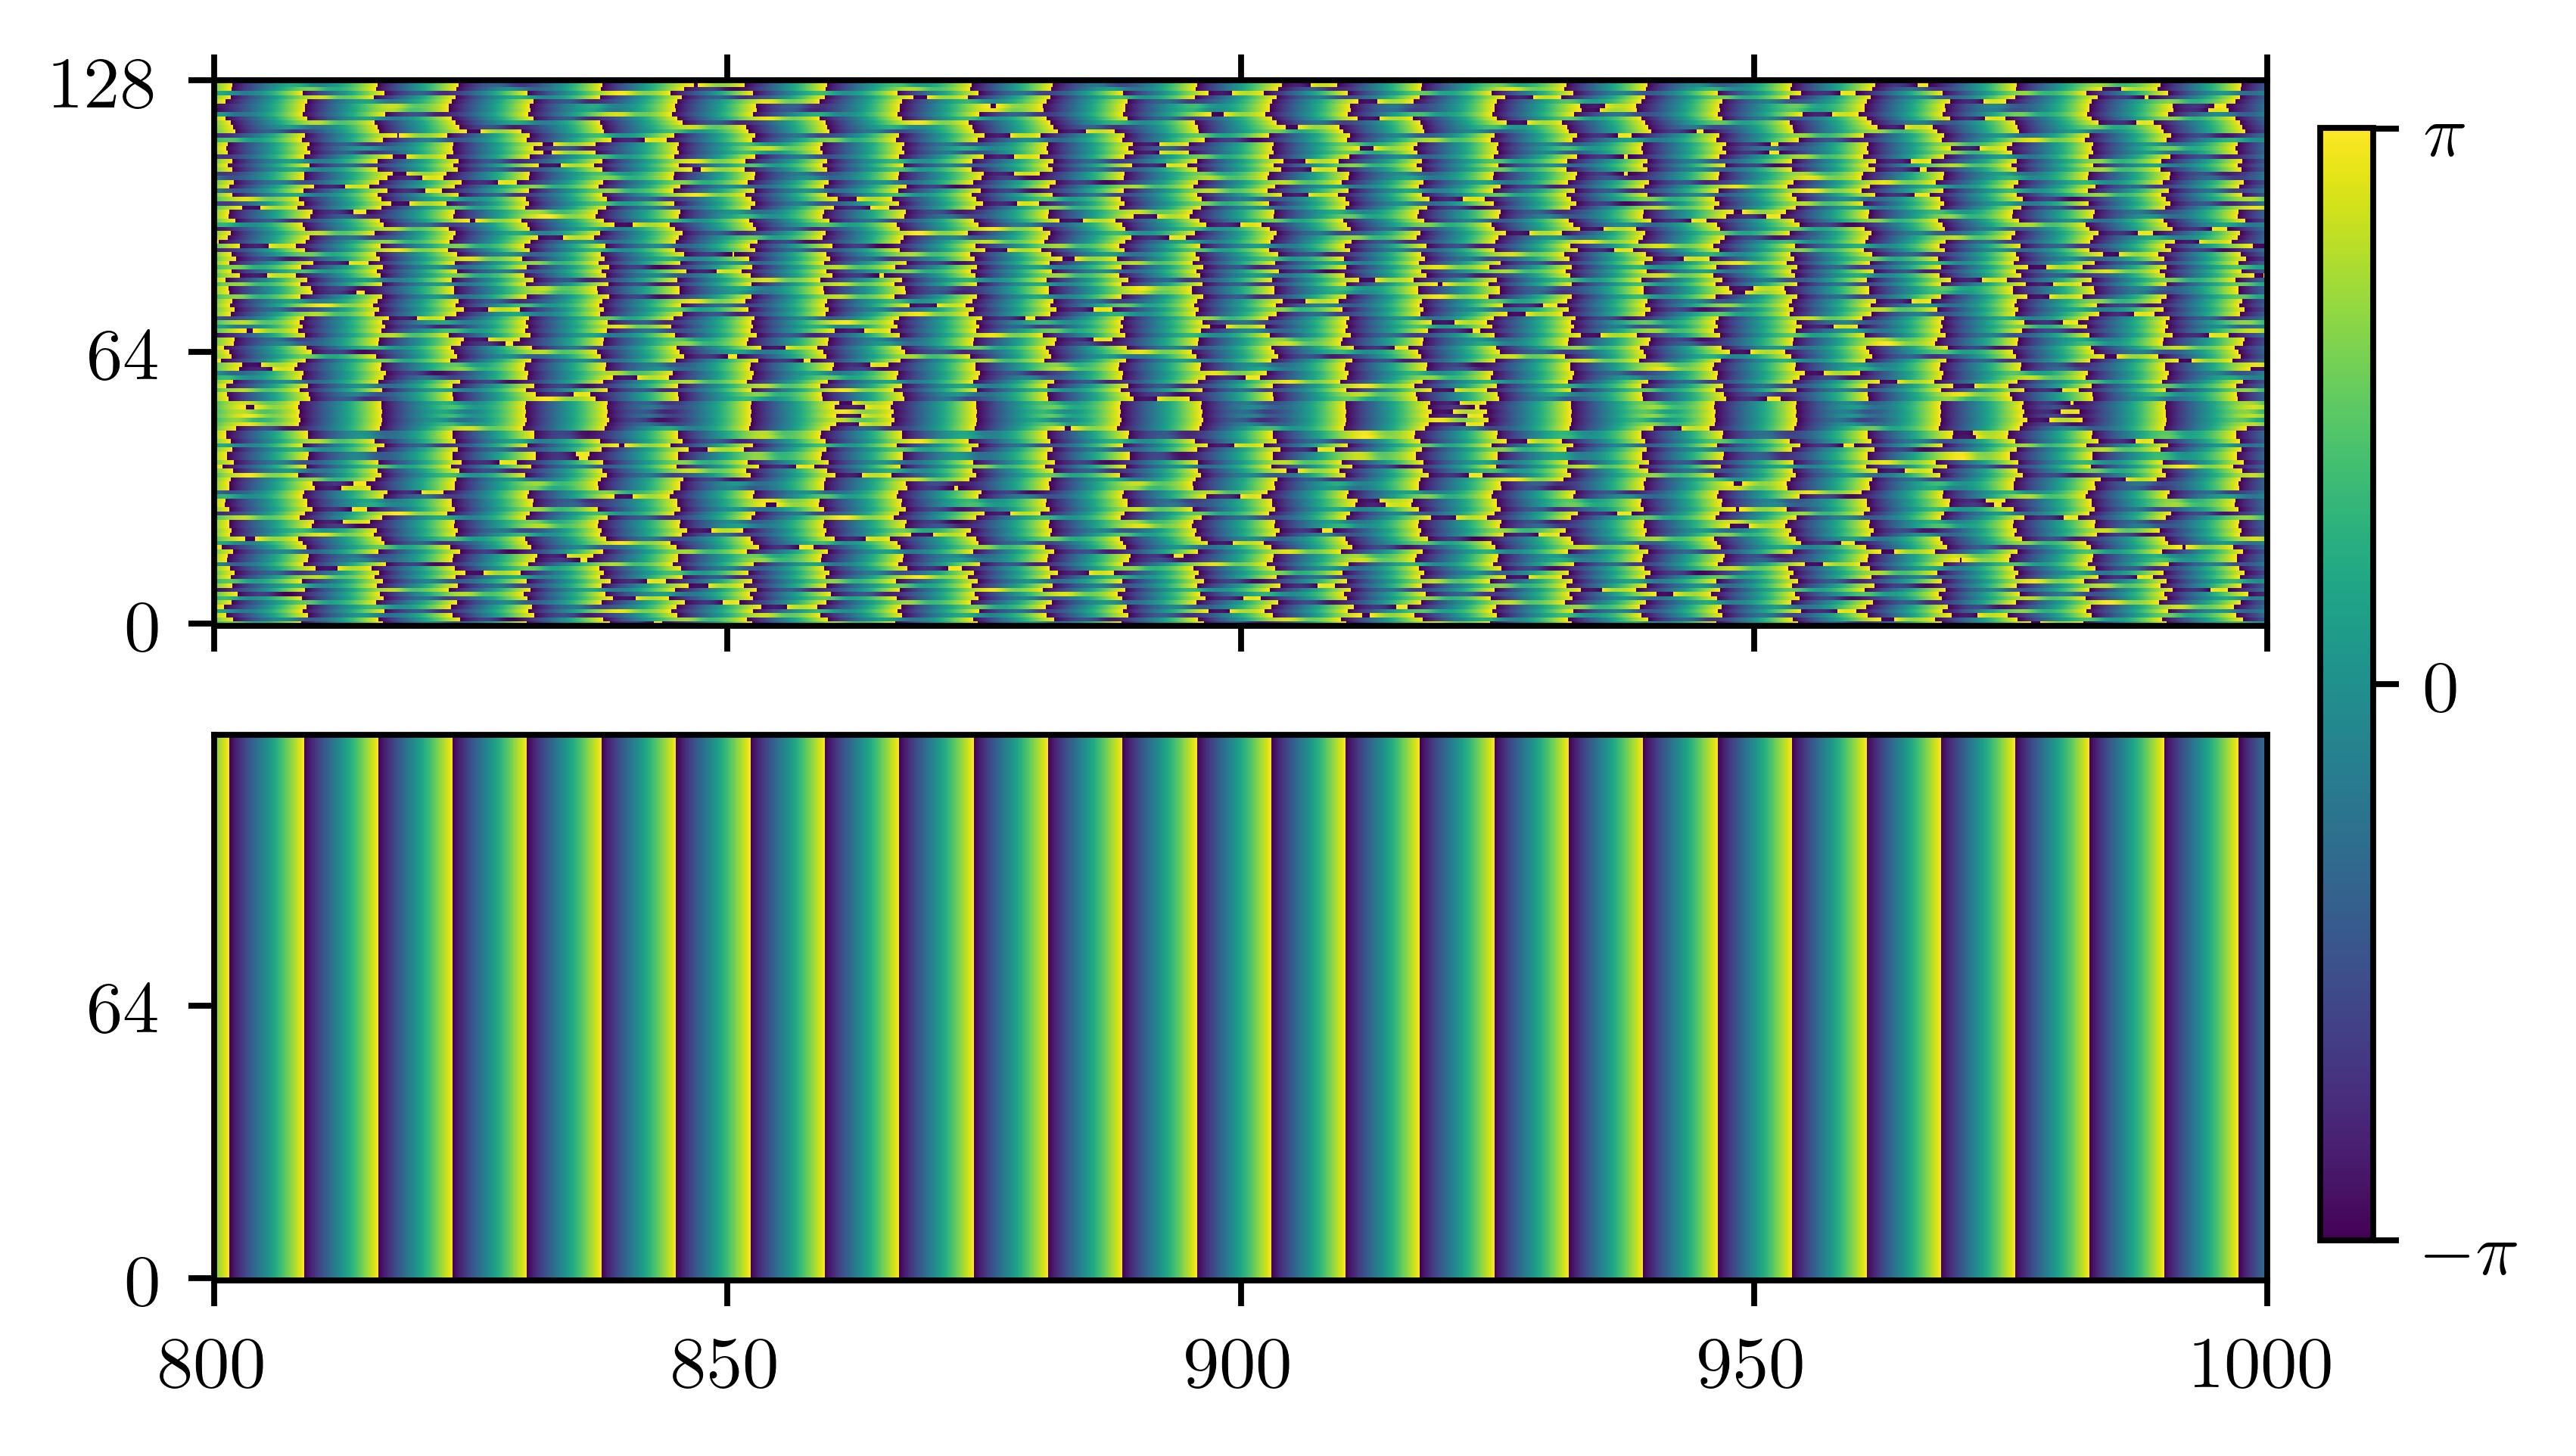
\includegraphics[width=0.99\textwidth]{figure/abrams_overhead}
        \caption{}
        \label{fig:abrams_overhead}
      \end{subfigure}%
      \begin{subfigure}{0.33\columnwidth}
        \centering
        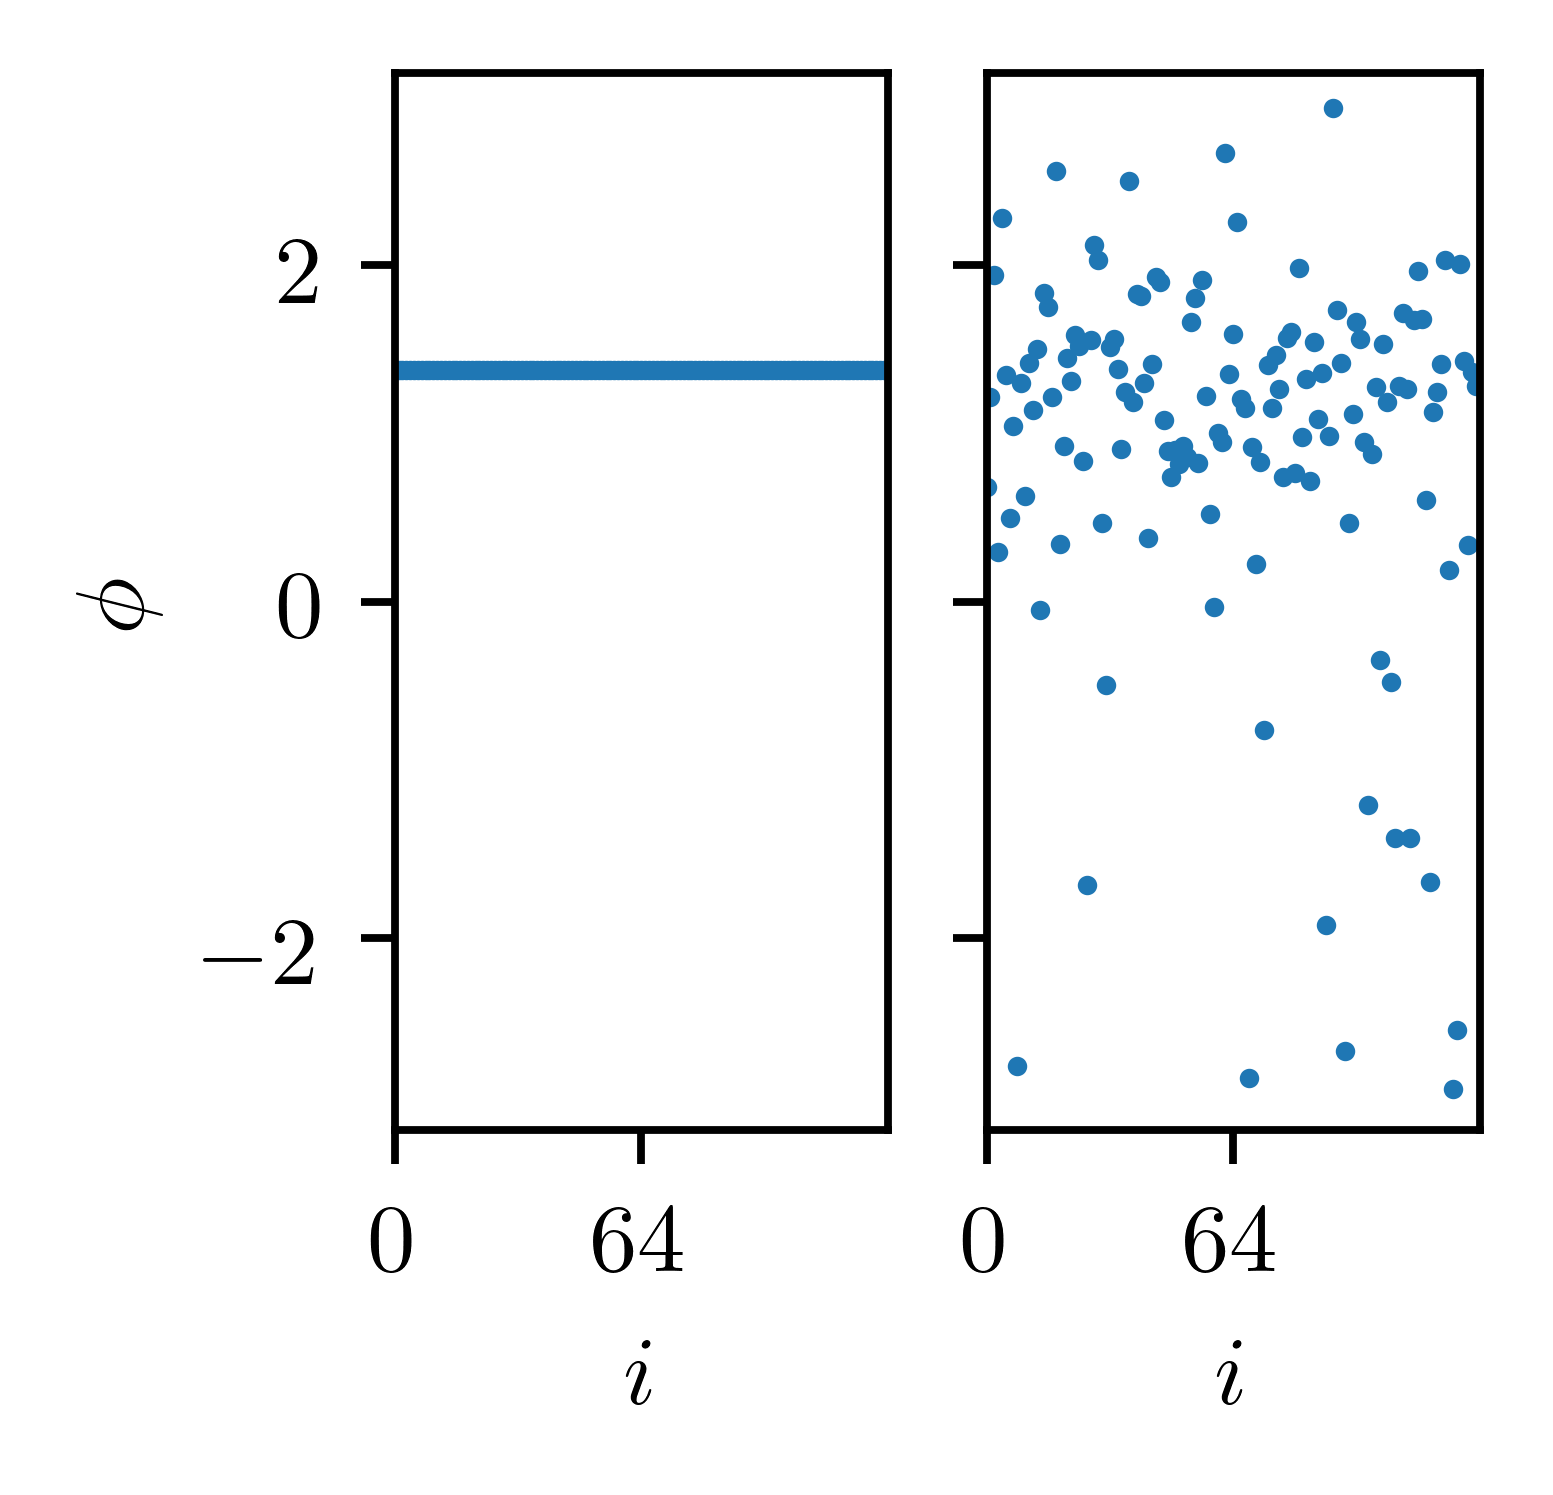
\includegraphics[width=0.99\textwidth]{figure/abrams_snapshot}
        \caption{}
        \label{fig:abrams_snapshot}
      \end{subfigure}%
      \caption{(a) A time series of a chimeric system, with an asynchronous population (above) and a synchronous population (below).
        (b) A snapshot of the chimeric system, with the synchronous population (left) and asynchronous population (right) separated.
      }
      \label{fig:abrams}
    \end{figure}
    The time average of the variance between groups of a system's order parameter provides a good measure for how chimeric it is \cite{Shanahan2010}.
    The \textbf{chimera-like index} is given by $\chimera = \expval{\sigma_{\text{chi}}}_{T}$
    where
    \begin{equation}
      \label{eq:chimera}
      \sigma_{\text{chi}}(t)
      =
      \frac{1}{M - 1} \sum_{c \in C}{\pqty{\ordparam_{c}(t) - \expval{\ordparam_{c}}_{C}}}^{2}
    \end{equation}
    and $\ordparam(t) = \abs{\expval{e^{i \phase_{k}(t)}}_{k \in C}}$ is a measure of the synchrony of the phases of oscillators within a community $C$.

    \section{Seizures}
    \textbf{Seizures} are abnormally synchronous electrical activity in the brain \cite{Kandel2013}.
    They often present as trances or convulsions, and chronically affect about \SI{3}{\percent} of the United States population.
    \textbf{Focal seizures} are seizures limited to a small portion of the brain.
    As they are a subsection of the brain oscillating synchronously while the rest oscillates asynchronously, they often present in models as chimera states.

    \section{The Model}
    This research used a network of modified Hindmarsh-Rose neurons \cite{Santos2017}:
    \begin{align}
      \label{eq:hr_x}
      \begin{split}
      \dot{\hrx}_{j}
      ={}&
        \hry_{j}
        -
        \hrx_{j}^{3}
        +
        b \hrx_{j}^{2}
        +
        I_{j}
        -
        \hrz_{j} \\
        &\quad -
        \frac{\hra}{n'_{j}} \sum_{k ={} 1}^{N} G'_{j k} \Theta_{j}(\hrx_{k}) \\
        &\qquad -
        \frac{\hrb}{n''_{j}} \sum_{k ={} 1}^{N} G''_{j k} \Theta_{j}(\hrx_{k})
      \end{split} \\
      \label{eq:hr_y}
      \dot{\hry}_{j}
      ={}&
        1
        -
        5 \hrx_{j}^{2}
        -
        \hry_{j} \\
      \label{eq:hr_z}
      \dot{\hrz}_{j}
      ={}&
        \mu \pqty{s \bqty{\hrx_{j} - \hrx_{\text{rest}}} - \hrz_{j}}
    \end{align}
    where $\Theta_{j}(\hrx_{k})
      =
      \frac{\hrx_{j} - \hrx_{\text{rev}}}{1 + \exp(-\lambda \bqty{\hrx_{k} - \theta})}$.
      The model was integrated for various values of $\hra$ and $\hrb$.
      \Cref{tab:hr_params} shows the values and meanings of the symbols in the model.

      \begin{table}[ht]
        \centering
        {\small
        \begin{tabular}{p{1in} | p{1in} | p{5in}}
          Symbol & Value & Meaning \\ \hline
          $\hrx_{j}$ & --- & Membrane potential of the $j$th neural mass \\
          $\hry_{j}$ & --- & Associated with the fast processes \\
          $\hrz_{j}$ & --- & Associated with slow processes \\ \hline
          $b$ & 3.2 & Tunes the spiking frequency \\
          $I_{j}$ & 4.4 & External input current \\
          $\hrx_{\text{rev}}$ & 2 & Ambient reverse potential \\
          $\lambda$ & 10 & Sigmoidal activation function parameter \\
          $\theta$ & -0.25 & Sigmoidal activation function parameter \\
          $\mu$ & 0.01 & Time scale for variation of $z$ \\
          $s$ & 4 & Governs adaptation \\
          $\hrx_{\text{rest}}$ & -1.6 & Resting/equilibrium potential \\ \hline
          $\hra$ & Varied & Connection strength within cortices \\
          $n_{j}'$ & \Cref{fig:connectome_matrix} & Number of connections within a cortex from the $j$th neuron \\
          $G_{j k}'$ & \Cref{fig:connectome_matrix} & Intra-cortical connection matrix \\
          $\hrb$ & Varied & Connection strength between cortices \\
          $n_{j}''$ & \Cref{fig:connectome_matrix} & Number of connections between cortices from the $j$th neuron \\
          $G_{j k}''$ & \Cref{fig:connectome_matrix} & Inter-cortical connection matrix
        \end{tabular}
        \caption[Hindmarsh-Rose Parameters]{The list of parameters used in modeling the Hindmarsh-Rose network.}
        \label{tab:hr_params}
        }
      \end{table}


    \section{The Network}
    The oscillator network (\cref{fig:connectome}) was modeled after the mouse connectome \cite{Oh2014}.
    \begin{figure}
      \centering
      \begin{subfigure}{0.49\columnwidth}
        \centering
        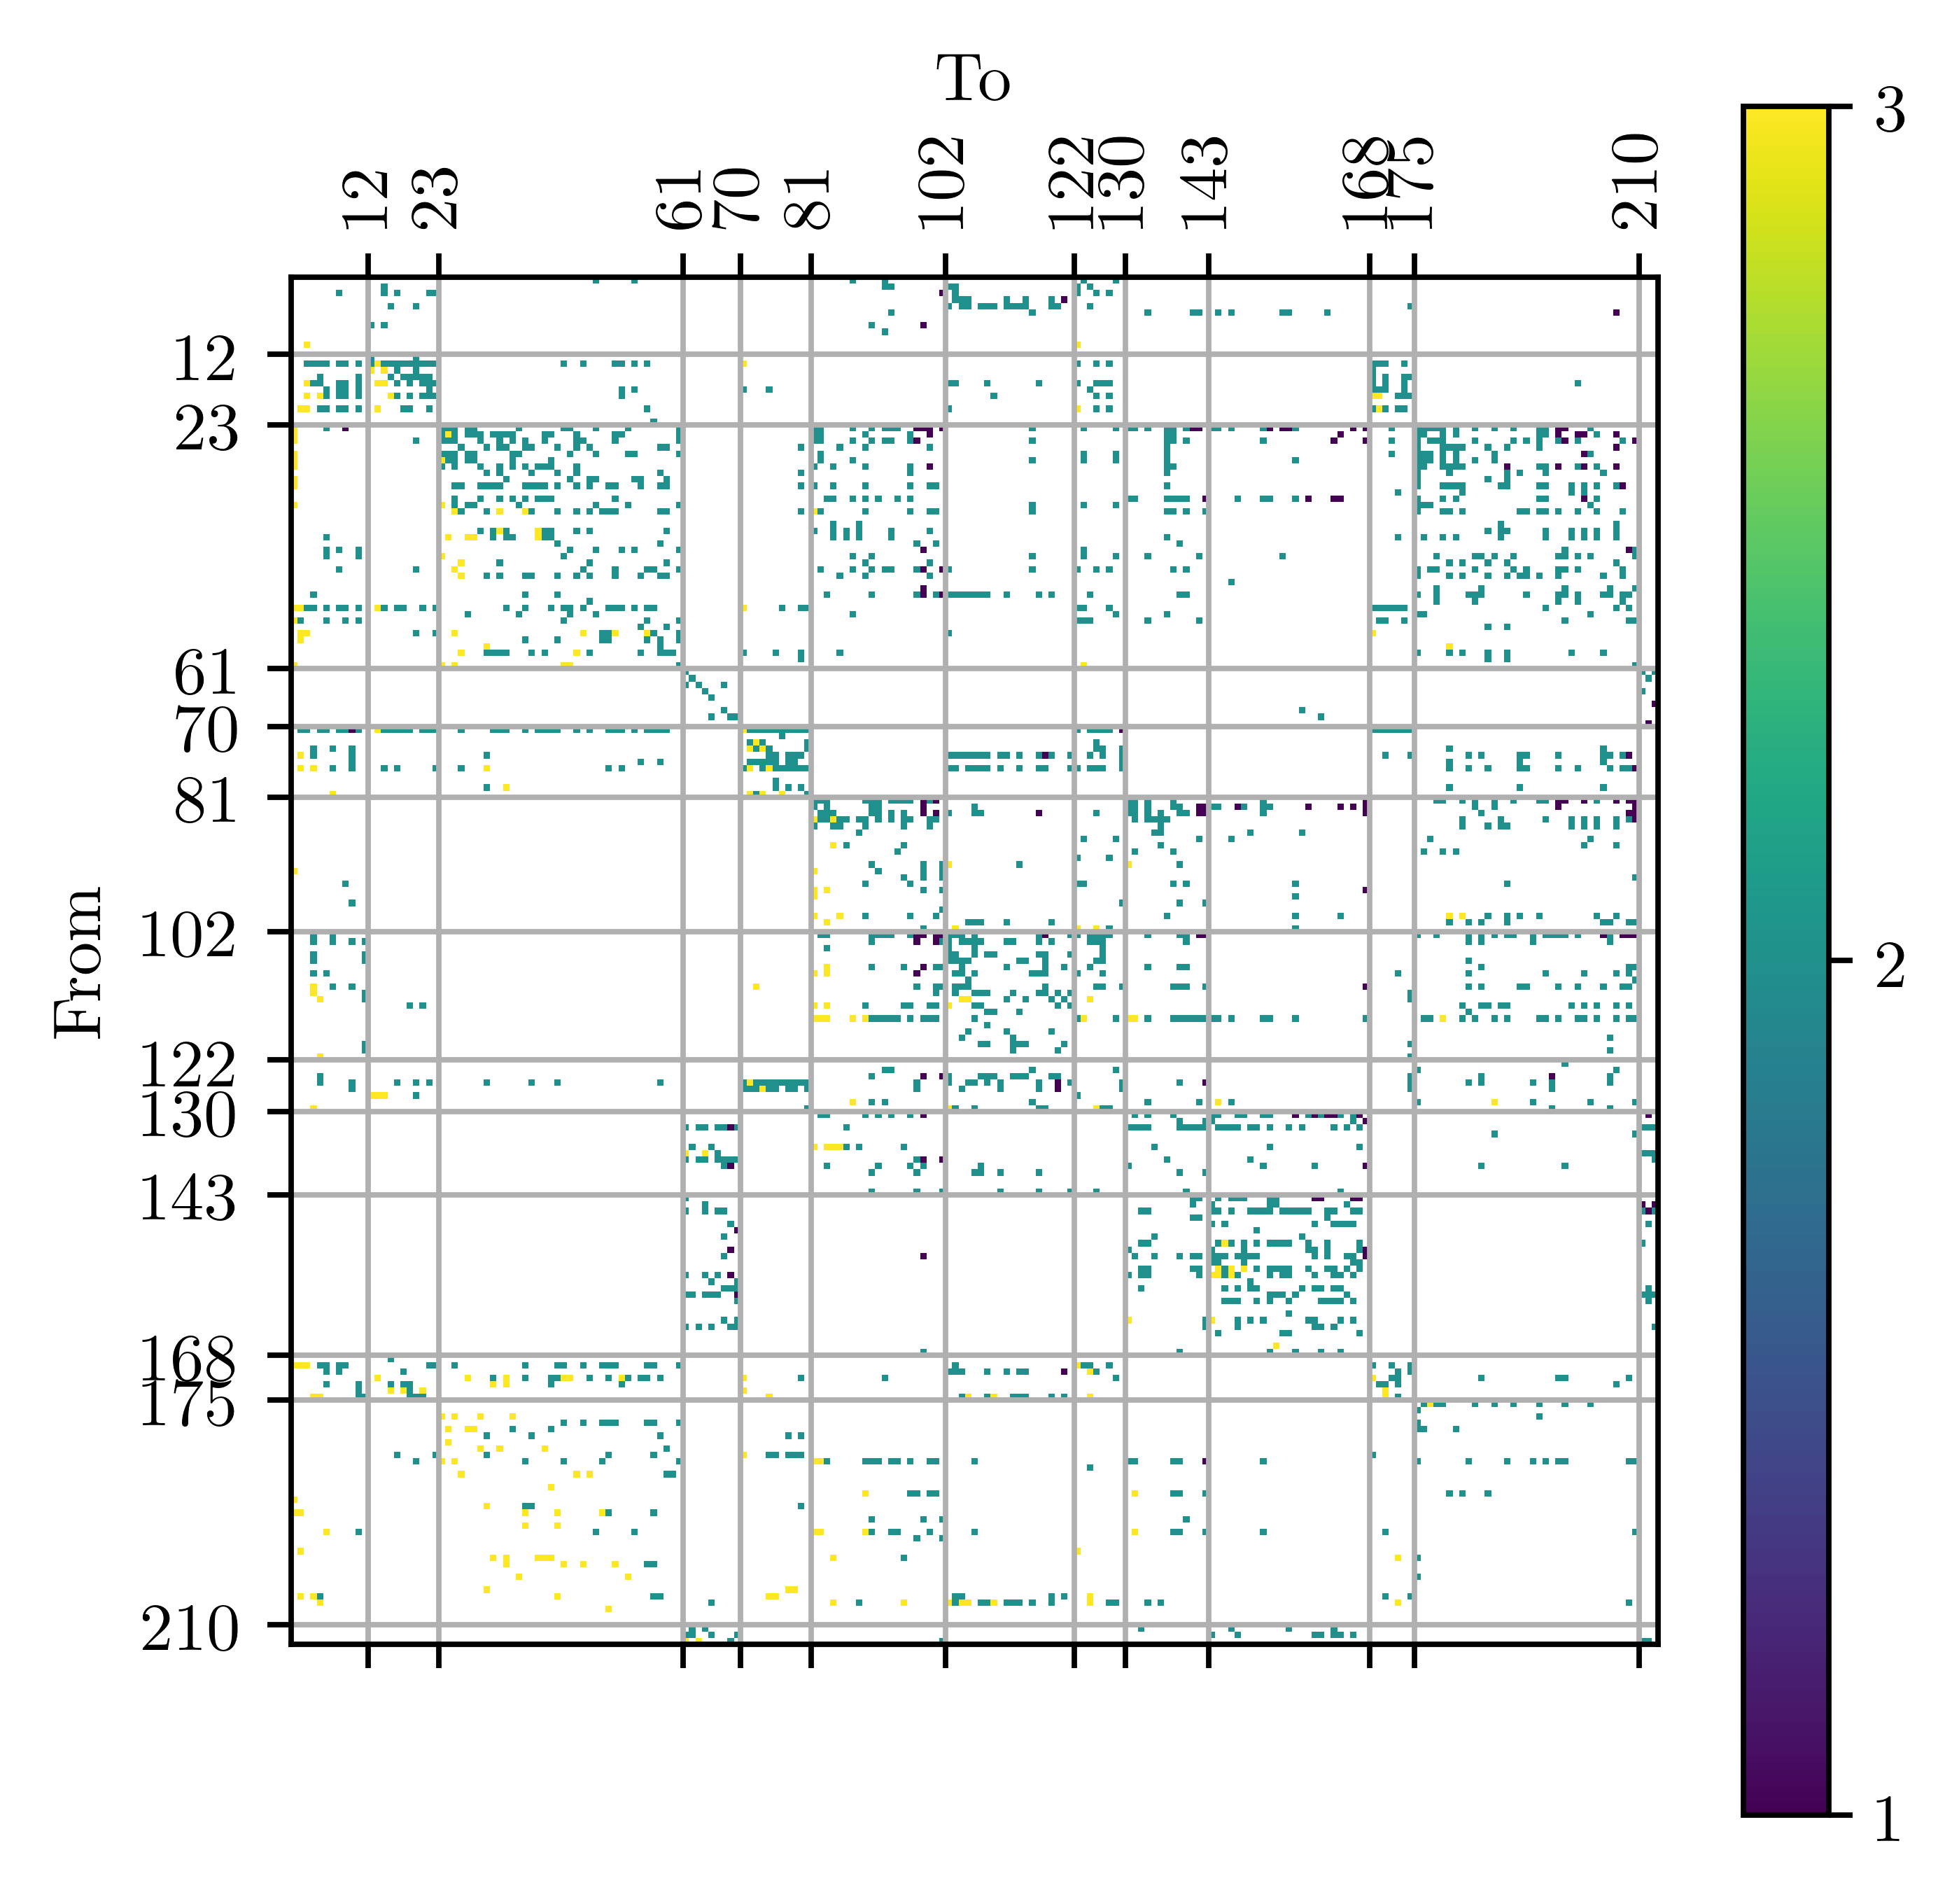
\includegraphics[width=0.99\textwidth]{figure/n}
        \caption{}
        \label{fig:connectome_matrix}
      \end{subfigure}%
      \begin{subfigure}{0.49\columnwidth}
        \centering
        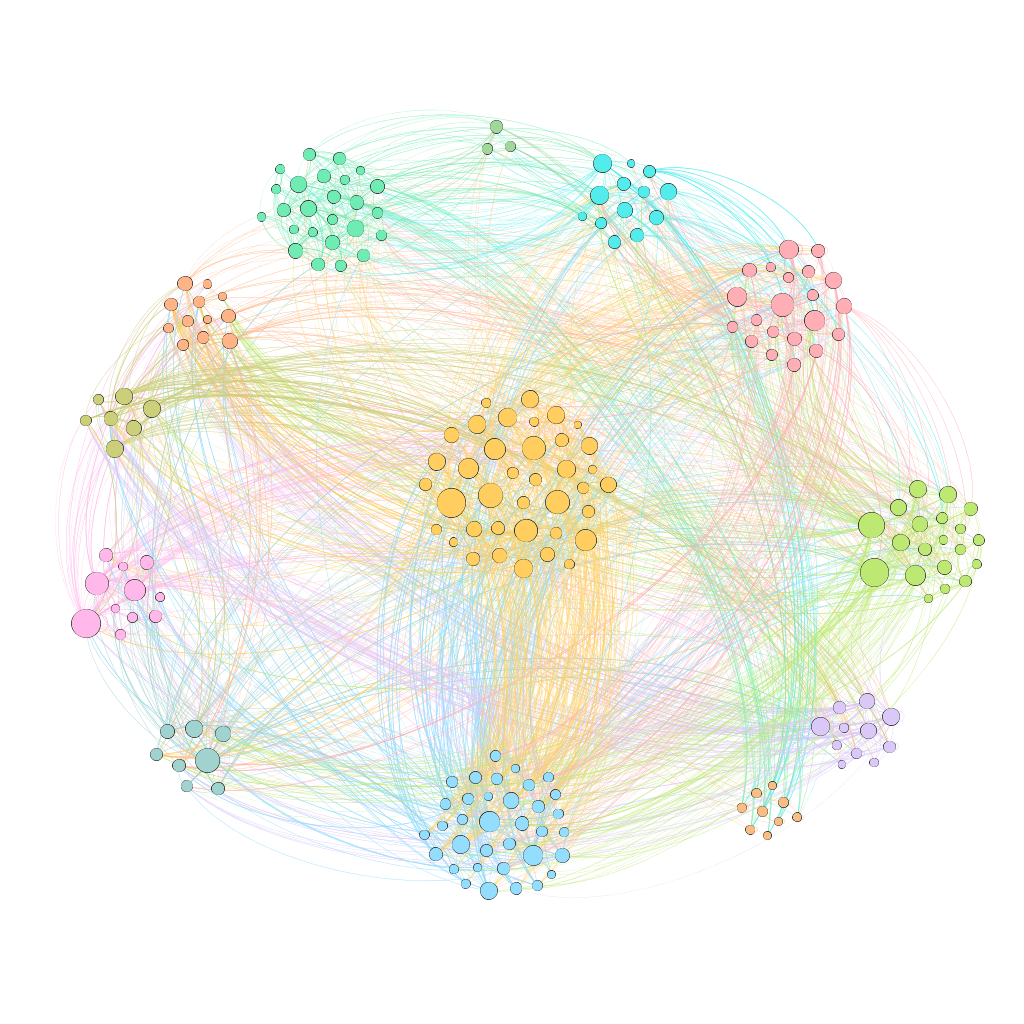
\includegraphics[width=0.99\textwidth]{figure/network}
        \caption{}
        \label{fig:connectome_embedding}
      \end{subfigure}
      \caption{(a) The mouse connectome represented as (a) a matrix and (b) a graph embedding.}
      \label{fig:connectome}
    \end{figure}

    \section{Chimera State Presence}
    Chimera states are more prevalent in the parts of parameter space where $\hra > \hrb$ (see \cref{fig:landscape}).
    This is unsurprising, as comparatively strong intra-community coupling is necessary for chimera states.
    The highly chimeric patch where $(\hra, \hrb) \in (0, 0.1) \times (0, 0.1)$ is worthy of further investigation.

    \section{Model Quality}
    The model produced waveforms which were qualitatively similar to mouse EEG recordings (\cref{fig:mean_608_267}).
    \begin{figure}[ht]
      \centering
      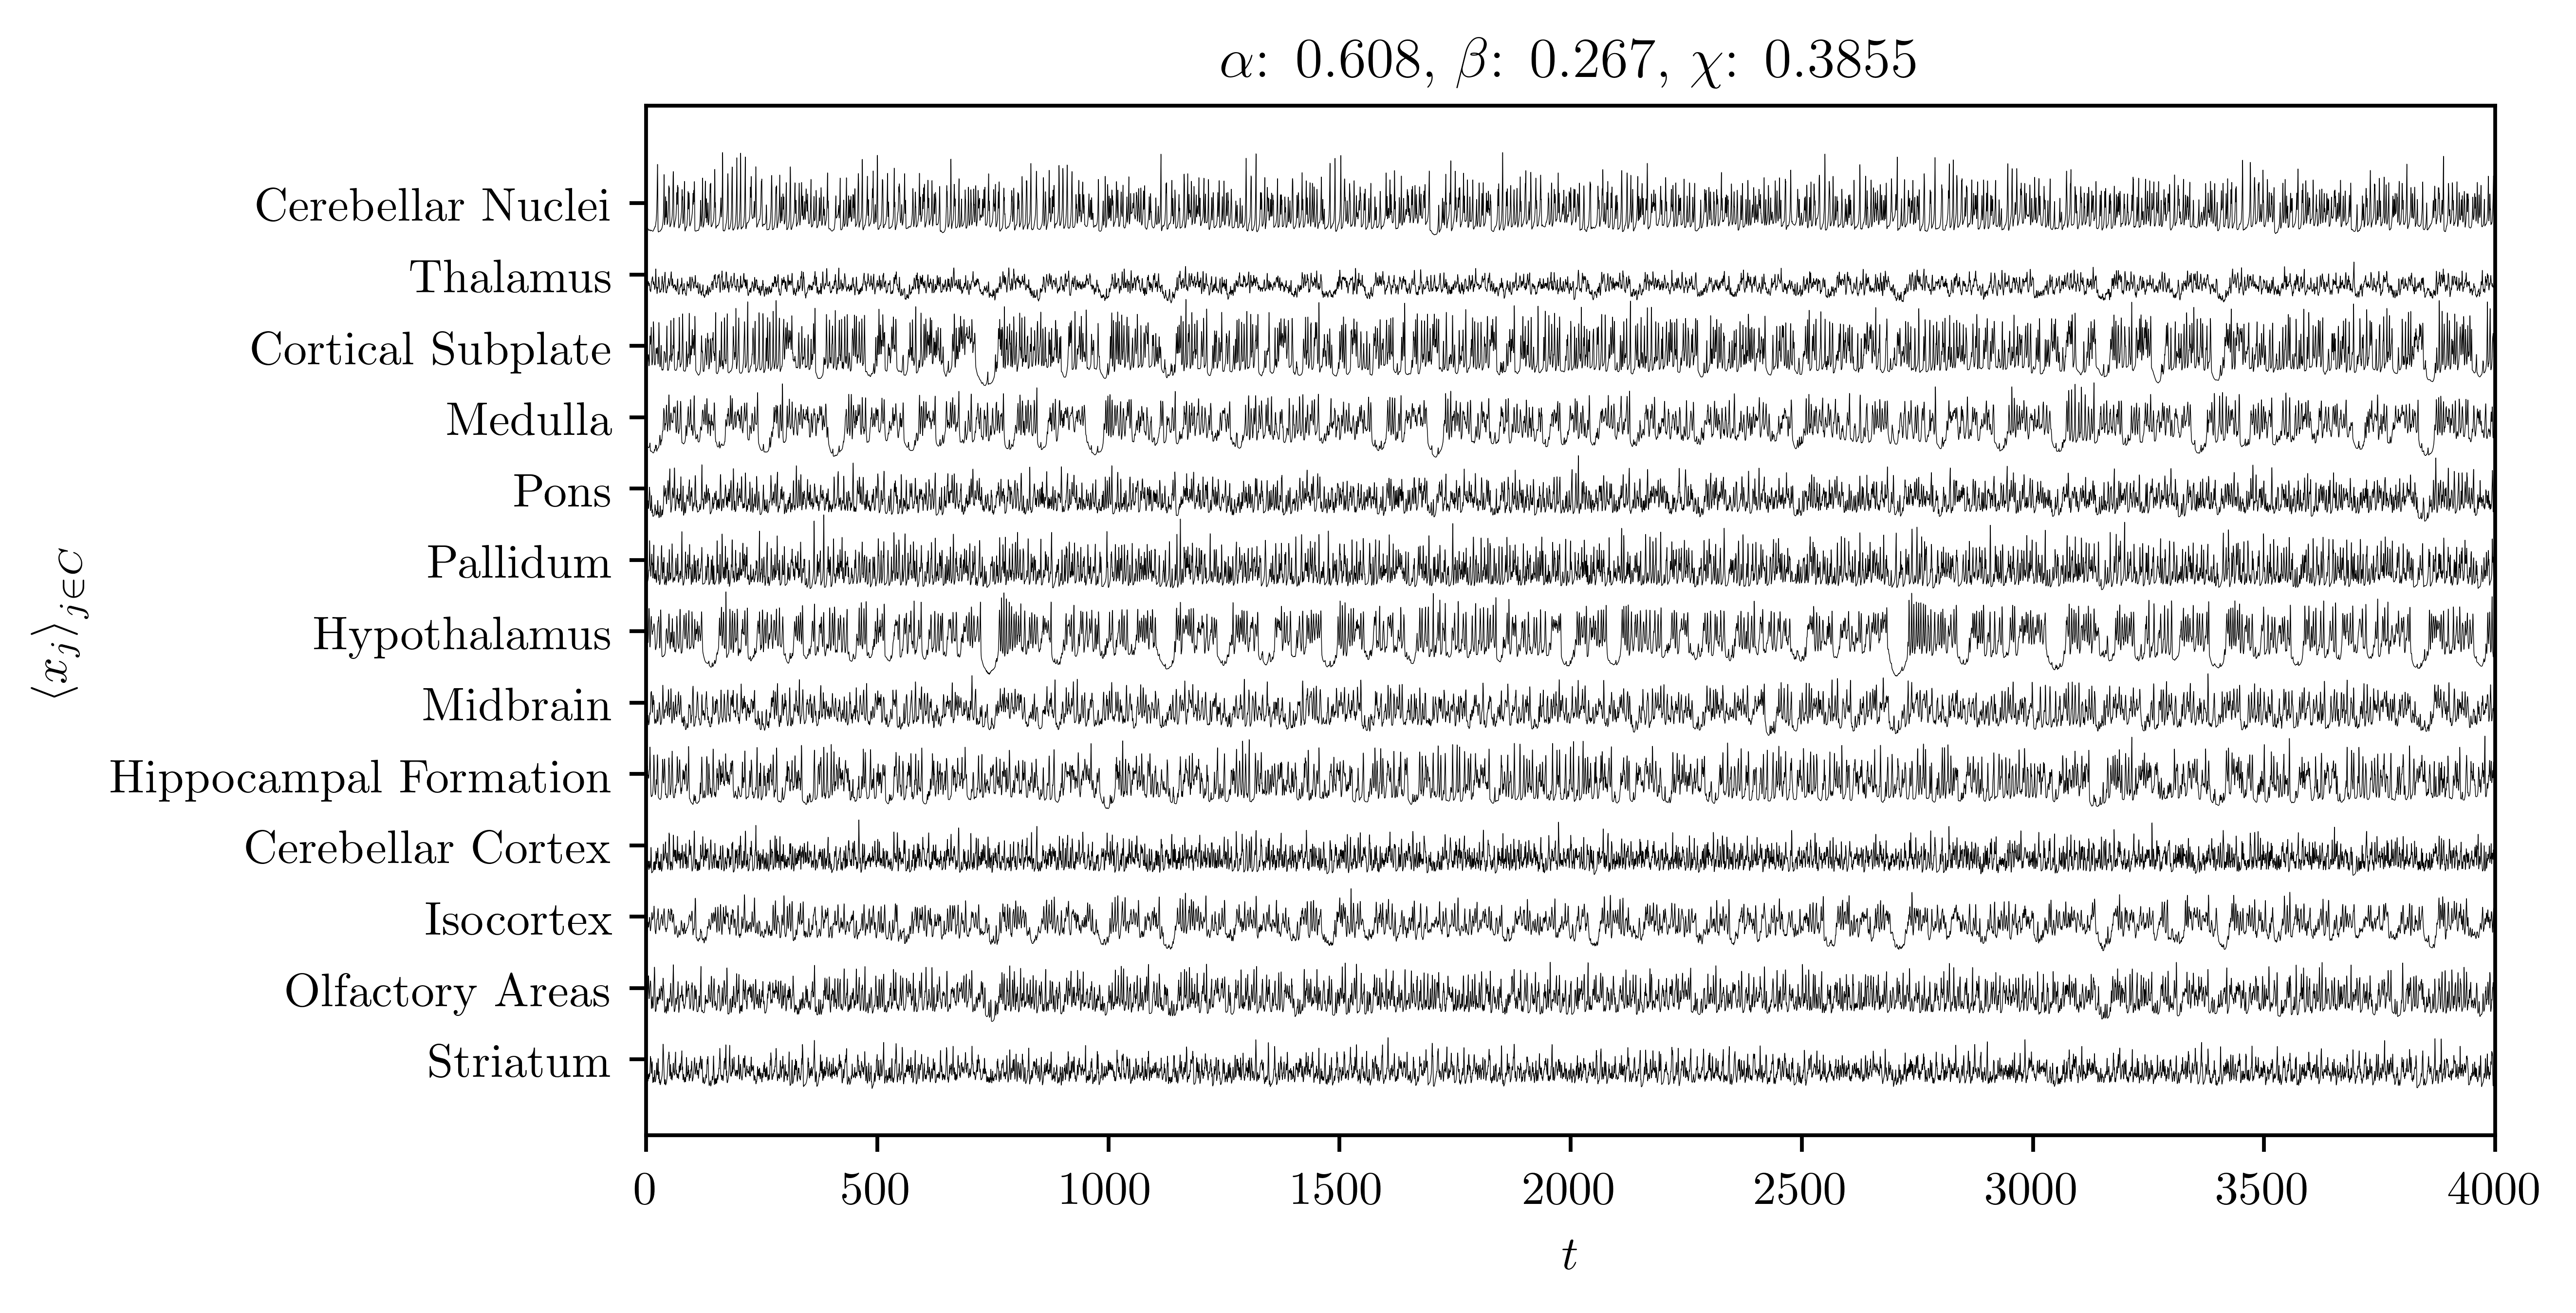
\includegraphics[width=0.99\columnwidth]{figure/means-0_608-0_267}
      \caption[Mean potential by cortex]{The mean membrane potential within each cortex.
        $\chimera$ is normalized to $\frac{1}{7}$.
      }
      \label{fig:mean_608_267}
    \end{figure}

    \section{Physical Region}
    For many parameter values, the neurons in the model never fired (shown in white in \cref{fig:landscape}).
    \begin{figure}
      \centering
    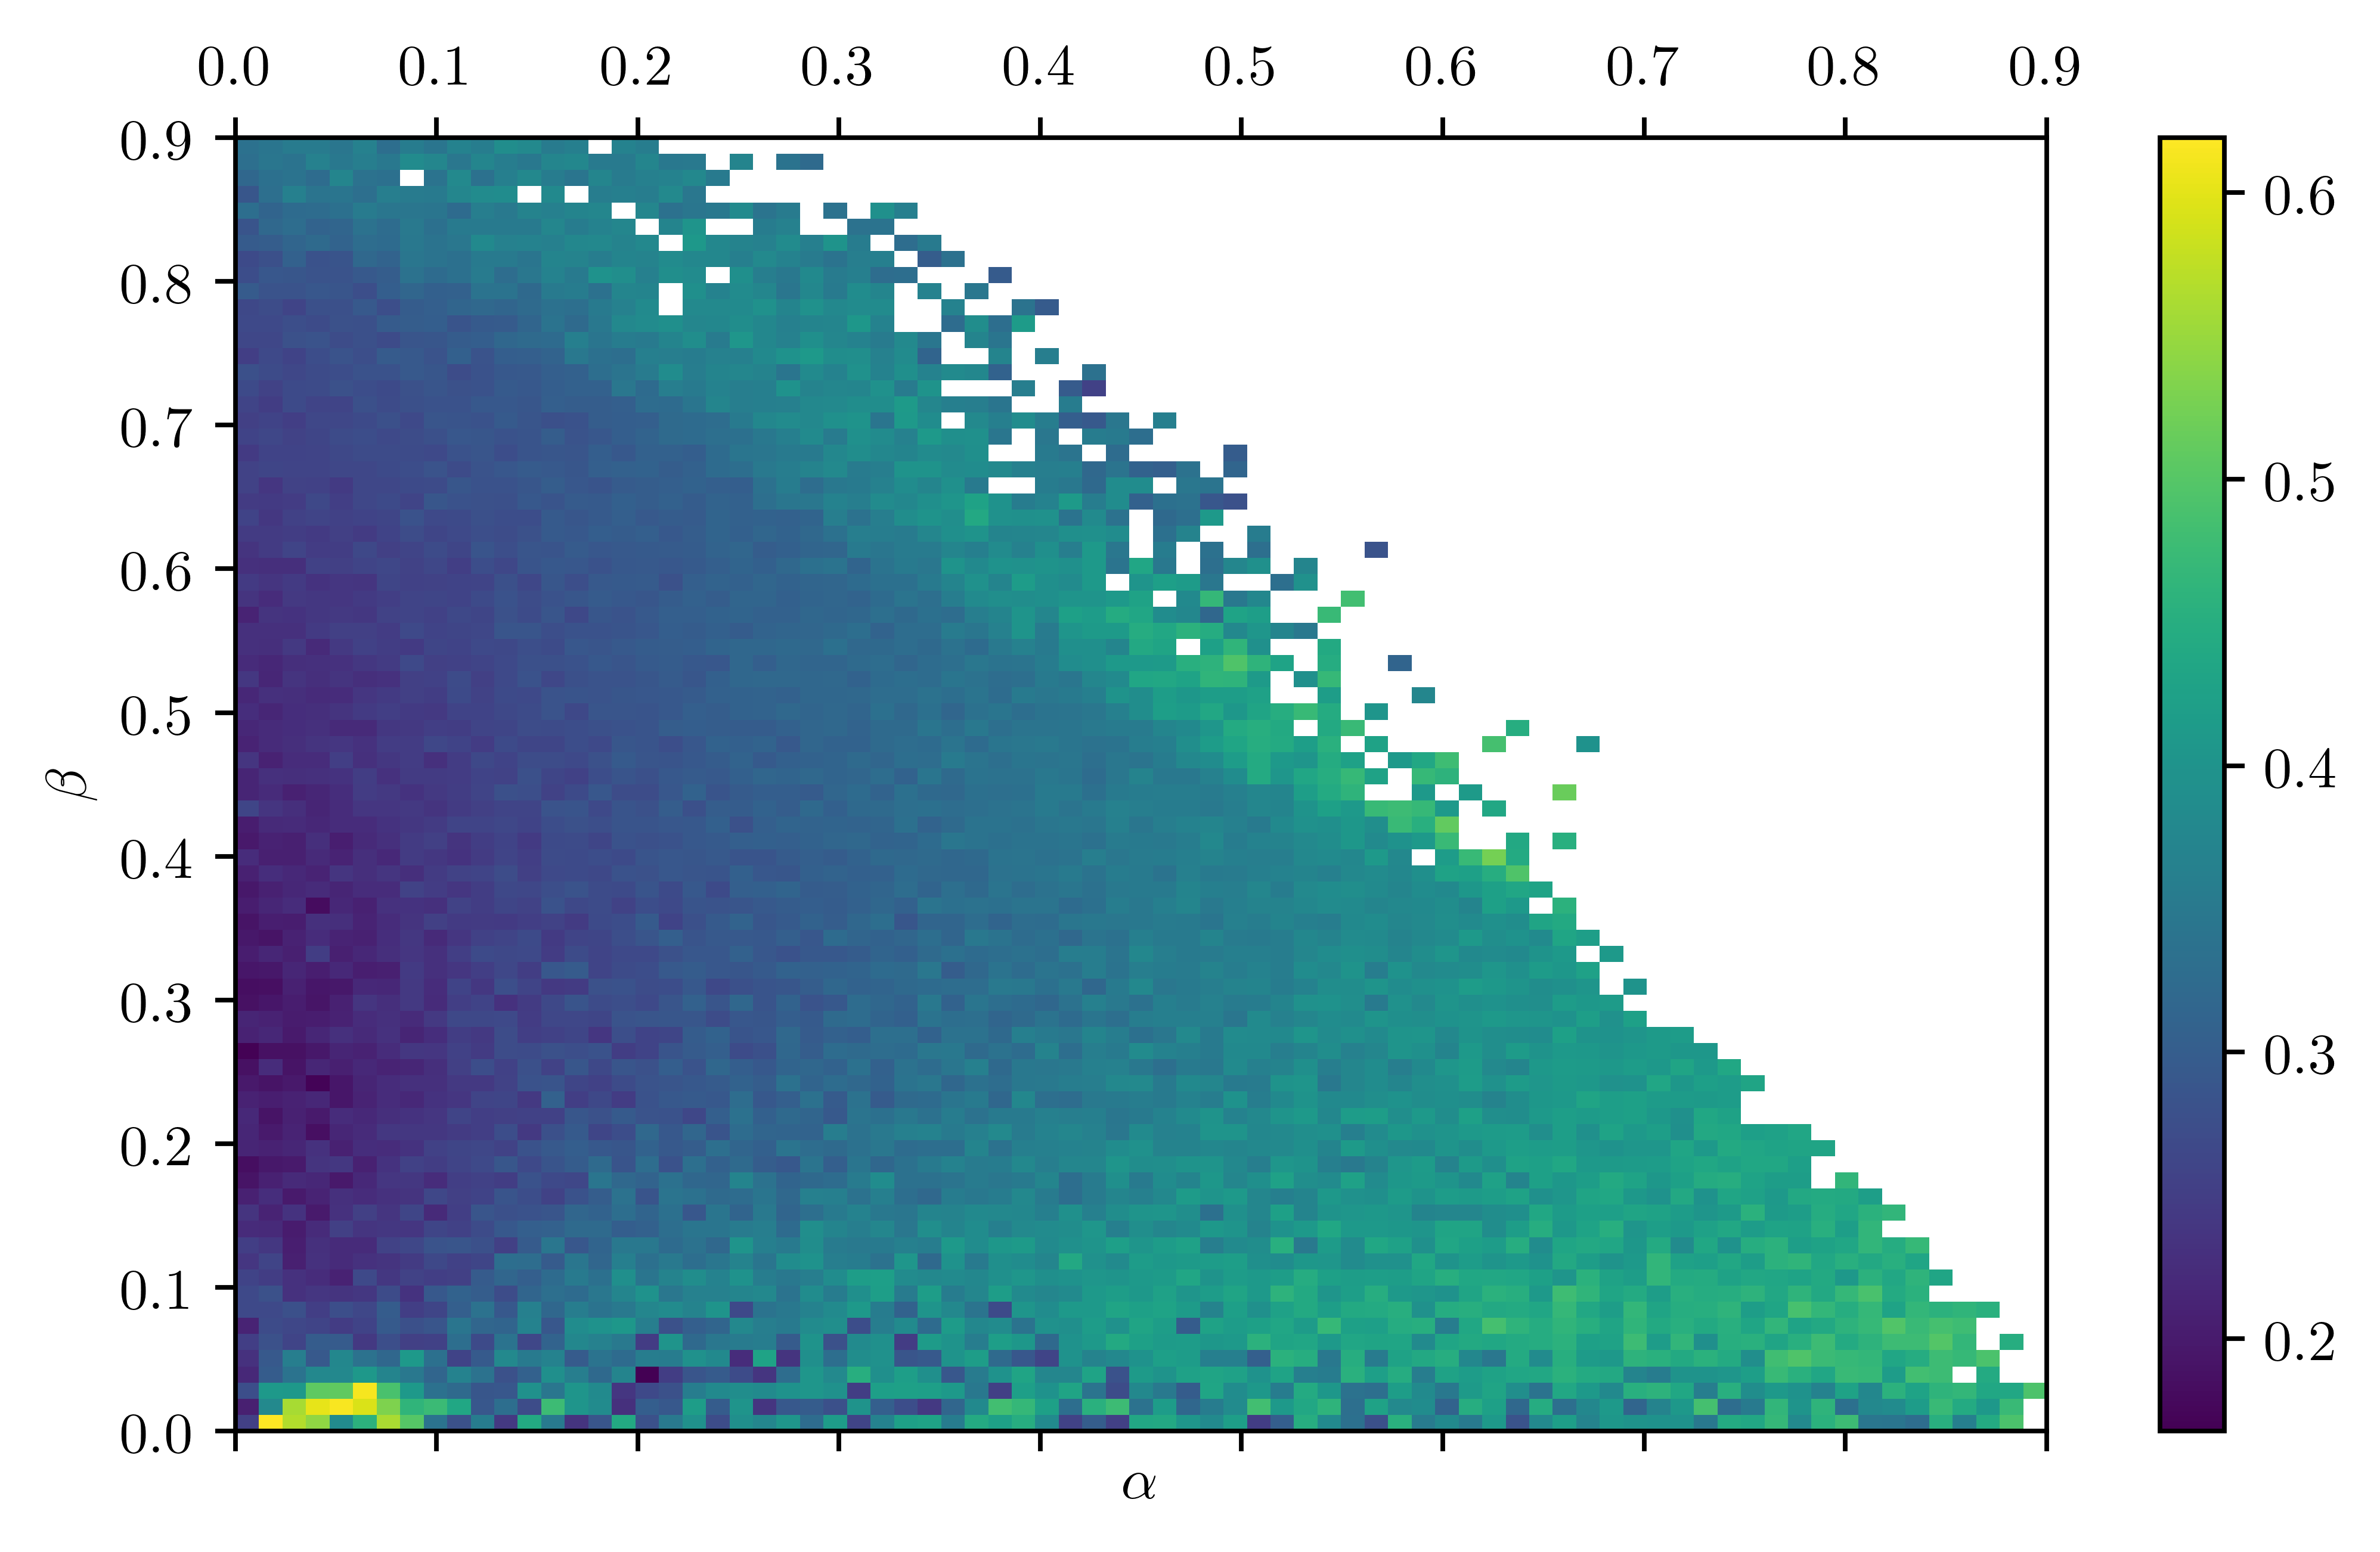
\includegraphics[width=\columnwidth]{figure/landscape}
      \caption{The normalized chimera-like index for the landscape of values of $\hra$ and $\hrb$.}
      \label{fig:landscape}
    \end{figure}
    The slope of the boundary between the physical and aphysical regions is negative, of a magnitude greater than 1.
    This indicates that $\hra$, the intra-cortical connection strength, has a stronger effect on the physicality of the model than $\hrb$ does.

    \section{Future Work}
    Further investigation of the exact nature of the boundary between the physical and aphysical regions would be beneficial.
    Additionally, a theoretical basis for the existence of the highly chimeric patch in
    $(\hra, \hrb) \in (0, 0.1) \times (0, 0.1)$
    would provide insight into the nature of these chimera states.


    \subsection{References}
    \begin{thebibliography}{99}
    \bibitem{Abrams2004} Daniel M. Abrams and Steven H. Strogatz. ``Chimera States for Coupled Oscillators''.
      In: \textit{Physical Review Letters} 93.17 (2004)

    \bibitem{Kuramoto2002} Yoshiki Kuramoto and Dorjsuren Battogtokh. ``Coexistence of Coherence and Incoherence in Nonlocally Coupled Phase Oscillators''.
      In: \textit{arXiv e-prints} cond-mat/0210694 (2002)

    \bibitem{Kandel2013} Eric R. Kandel. ``Principles of Neural Science'' Fifth ed., pp. 1116-1139. (2013)

    \bibitem{Oh2014} Seung Wook Oh et al. ``A Mesoscale Connectome of the Mouse Brain''.
      In: \textit{Nature} 508.7495 (2014)

    \bibitem{Santos2017} M.S. Santos et al. ``Chimera-like States in a Neuronal Network Model of the Cat Brain''.
      In: \textit{Chaos, Solitons \& Fractals} 101 (2017)

    \bibitem{Shanahan2010} Murray Shanahan. ``Metastable Chimera States in Community-Structured Oscillator Networks''.
      In: \textit{Chaos} 20.1 (2010)

    \end{thebibliography}


    \vspace{\fill}
    
\includegraphics[width=\columnwidth]{figure/UVM}
  \end{multicols}

\end{frame}

\end{document}

%%% Local Variables:
%%% mode: latex
%%% TeX-master: t
%%% End:
